\documentclass{article}\usepackage[]{graphicx}\usepackage[]{xcolor}
% maxwidth is the original width if it is less than linewidth
% otherwise use linewidth (to make sure the graphics do not exceed the margin)
\makeatletter
\def\maxwidth{ %
  \ifdim\Gin@nat@width>\linewidth
    \linewidth
  \else
    \Gin@nat@width
  \fi
}
\makeatother

\definecolor{fgcolor}{rgb}{0.345, 0.345, 0.345}
\newcommand{\hlnum}[1]{\textcolor[rgb]{0.686,0.059,0.569}{#1}}%
\newcommand{\hlsng}[1]{\textcolor[rgb]{0.192,0.494,0.8}{#1}}%
\newcommand{\hlcom}[1]{\textcolor[rgb]{0.678,0.584,0.686}{\textit{#1}}}%
\newcommand{\hlopt}[1]{\textcolor[rgb]{0,0,0}{#1}}%
\newcommand{\hldef}[1]{\textcolor[rgb]{0.345,0.345,0.345}{#1}}%
\newcommand{\hlkwa}[1]{\textcolor[rgb]{0.161,0.373,0.58}{\textbf{#1}}}%
\newcommand{\hlkwb}[1]{\textcolor[rgb]{0.69,0.353,0.396}{#1}}%
\newcommand{\hlkwc}[1]{\textcolor[rgb]{0.333,0.667,0.333}{#1}}%
\newcommand{\hlkwd}[1]{\textcolor[rgb]{0.737,0.353,0.396}{\textbf{#1}}}%
\let\hlipl\hlkwb

\usepackage{framed}
\makeatletter
\newenvironment{kframe}{%
 \def\at@end@of@kframe{}%
 \ifinner\ifhmode%
  \def\at@end@of@kframe{\end{minipage}}%
  \begin{minipage}{\columnwidth}%
 \fi\fi%
 \def\FrameCommand##1{\hskip\@totalleftmargin \hskip-\fboxsep
 \colorbox{shadecolor}{##1}\hskip-\fboxsep
     % There is no \\@totalrightmargin, so:
     \hskip-\linewidth \hskip-\@totalleftmargin \hskip\columnwidth}%
 \MakeFramed {\advance\hsize-\width
   \@totalleftmargin\z@ \linewidth\hsize
   \@setminipage}}%
 {\par\unskip\endMakeFramed%
 \at@end@of@kframe}
\makeatother

\definecolor{shadecolor}{rgb}{.97, .97, .97}
\definecolor{messagecolor}{rgb}{0, 0, 0}
\definecolor{warningcolor}{rgb}{1, 0, 1}
\definecolor{errorcolor}{rgb}{1, 0, 0}
\newenvironment{knitrout}{}{} % an empty environment to be redefined in TeX

\usepackage{alltt}
\usepackage{amsmath} %This allows me to use the align functionality.
                     %If you find yourself trying to replicate
                     %something you found online, ensure you're
                     %loading the necessary packages!
\usepackage{amsfonts}%Math font
\usepackage{graphicx}%For including graphics
\usepackage{hyperref}%For Hyperlinks
\usepackage[shortlabels]{enumitem}% For enumerated lists with labels specified
                                  % We had to run tlmgr_install("enumitem") in R
\hypersetup{colorlinks = true,citecolor=black} %set citations to have black (not green) color
\usepackage{natbib}        %For the bibliography
\setlength{\bibsep}{0pt plus 0.3ex}
\bibliographystyle{apalike}%For the bibliography
\usepackage[margin=0.50in]{geometry}
\usepackage{float}
\usepackage{multicol}

%fix for figures
\usepackage{caption}
\newenvironment{Figure}
  {\par\medskip\noindent\minipage{\linewidth}}
  {\endminipage\par\medskip}
\IfFileExists{upquote.sty}{\usepackage{upquote}}{}
\begin{document}

\vspace{-1in}
\title{Lab 05 -- MATH 240 -- Computational Statistics}

\author{
  Yuliia Heleveria \\
  MATH 240 Lab A  \\
  Mathematics  \\
  {\tt yheleveria@colgate.edu}
}

\date{02/25/2025}

\maketitle

\begin{multicols}{2}
\begin{abstract}
We want to analyze the contributions of The Front Bottoms, Manchester Orchestra, and All Get Out to their collaborative song ``Allentown'' using audio analysis. Therefore, we created a batch file to speed up data collection of audio features. We extracted musical characteristics of .WAV files from three bands, including valence, instrumental and acoustic features, emotional impact, loudness, and lyrics analysis. We loaded and cleaned the data to perform statistical analysis for features of each band's tracks and their similarity with ``Allentown''. 
\end{abstract}

\noindent \textbf{Keywords:} Installing and using libraries; creating, cleaning, and merging data frames; statistical analysis; data visualization.

\section{Introduction}
``Allentown'' is a song released in 2018 by collaboration of The Front Bottoms and Manchester Orchestra and contributions from All Get Out. We would like to inspect which band made the most contribution to this song. We purchased all pre-``Allentown'' releases, totaling 181 tracks, including Allentown itself.
Using Essentia \citep{bogdanov2013essentia}, we extracted music data about given songs to determine the primary contributor to ``Allentown''. We summarized the style and characteristics of tracks, such as valence, arousal, emotions, and absence of voice or acoustic features, belonging to each band to determine stylistic features that resonate the most with ``Allentown''. 

Section 2 covers data collection and processing. Section 3 presents data analysis, and Section 4 discusses findings from comparing the stylistic features of three band's tracks with ``Allentown''.

\section{Methods}
We obtained Essentia models \citep{alonso2020tensorflow} of 181 songs for analysis. We used \texttt{stringr} package \citep{stringr} to create a batch file that creates command line prompts for each track. With the use of the batch file, we extracted data from .WAV files and then Essentia model for each track about features such as tempo in beats, average loudness, valence, arousal, aggressiveness, acoustic and instrumental sound. 

Using \texttt{jsonlite} package for \texttt{R} \citep{jsonlite}, we extracted stylistic features of provided songs. We loaded JSON files containing music analysis into \texttt{R} and extracted mean of spectral energy, dancebility, tempo in beats per minute, musical key, musical mode and duration of the track in seconds. We also used LIWC text analysis tool \citep{boyd2022development} to extract features that describe thoughts, feelings, and personality traits in the tracks. We merged the data frames and saved them as two .csv files, as training and testing data, combining lyrics and audio analysis. 

Using \texttt{tidyverse} package \citep{tidyverse}, we summarized data numerically for each feature of interest. We computed minimum, maximum, lower and upper fences for each tracks's feature for All Get Out, Manchester Orchestra, and The Front Bottoms to determine if ``Allentown'''s features are within range or outlying for each band's songs. Based of the statistical summaries, we computed visual aids by creating a table using \texttt{xtable} library \citep{xtable} and column plots using \texttt{tidyverse} to determine how ``Allentown'' differs from music of each band based on the count of how many features of ``Allentown'' are within range and out of range for each band.


\section{Results}
We analyzed stylistic features of ``Allentown'' in comparison to 180 tracks from the contributing bands. Out statistical summaries and visualizations (see Figure \ref{plot.allen}) show that Manchester Orchestra has the most similar musical features to ``Allentown'', depicting the band's major contribution to creation of the track. Manchester Orchestra has the largest number of features that ``Allentown'' is within the range of. Manchester Orchestra also has the fewest features that are out of range of ``Allentown''. The result suggest that while each band contributes unique stylistic features, Manchester Orchestra has influenced creation of ``Allentown'' the most.

\section{Discussion}
We performed preliminary data analysis by creating \texttt{boxplots} that represent relation of data from ``Allentown'' in comparison to median values of the same data collected from the three contributing artists. 
\texttt{Boxplots} comparing ``Allentown'' to media values of each band suggest artists' mixed influence on track's features, with Manchester Orchestra being most similar to ``Allentown'' in overall loudness. The Front Bottoms tracks have the median word count as ``Allentown'''s word count . In regard to aggressiveness, ``Allentown'' is the most similar to tracks by All Get Out. Each band adds distinct stylistic elements to ``Allentown'', but further analysis is needed to quantify their contributions.


%Code for creating an xtable and column plots

%code to process before graphs begin




%Code for creating boxplots to represent artist data






%Call the boxplots
\begin{figure}[H]
\begin{knitrout}\scriptsize
\definecolor{shadecolor}{rgb}{0.969, 0.969, 0.969}\color{fgcolor}
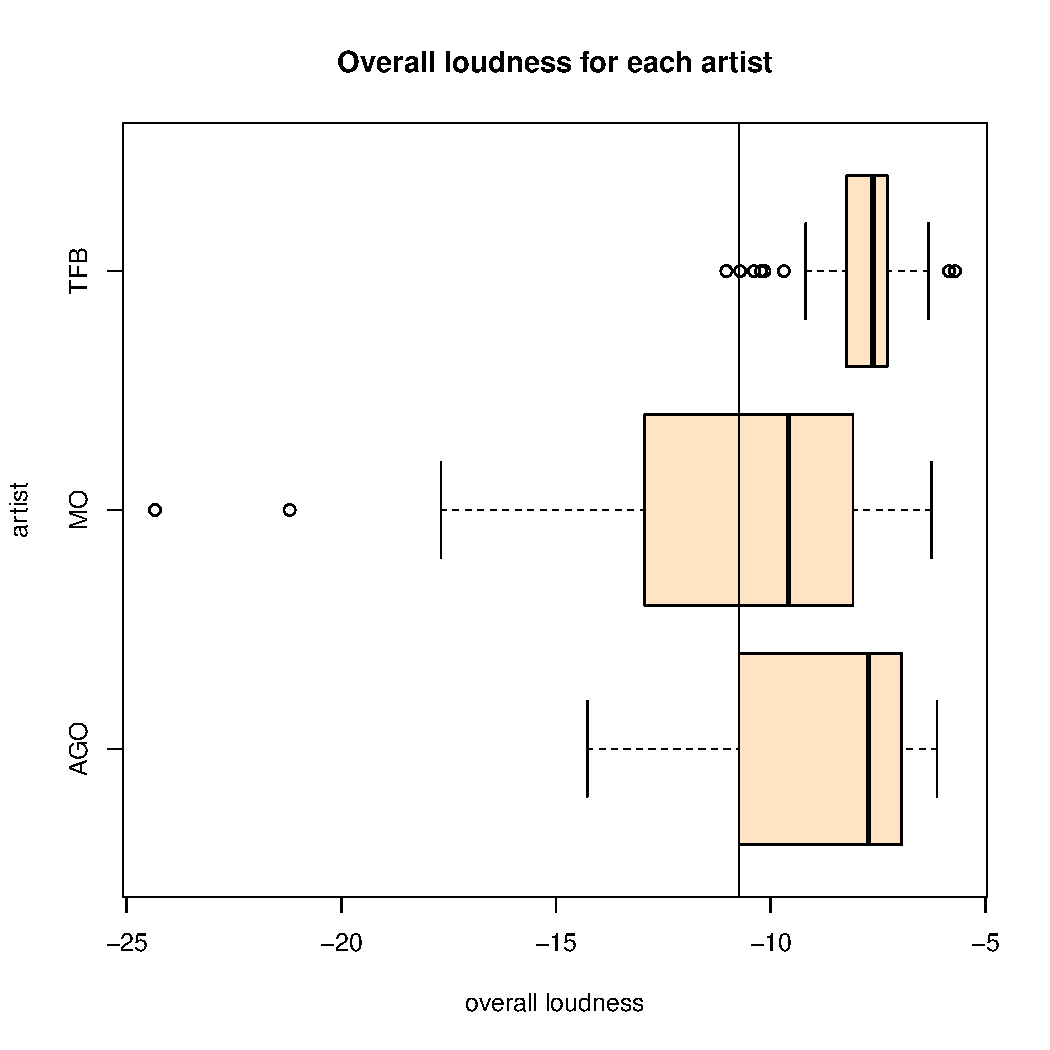
\includegraphics[width=\maxwidth]{figure/unnamed-chunk-3-1} 
\end{knitrout}
\caption{Vertical line represents ``Allentown''} \label{plot1}
\end{figure}

\begin{figure}[H]
\begin{knitrout}\scriptsize
\definecolor{shadecolor}{rgb}{0.969, 0.969, 0.969}\color{fgcolor}
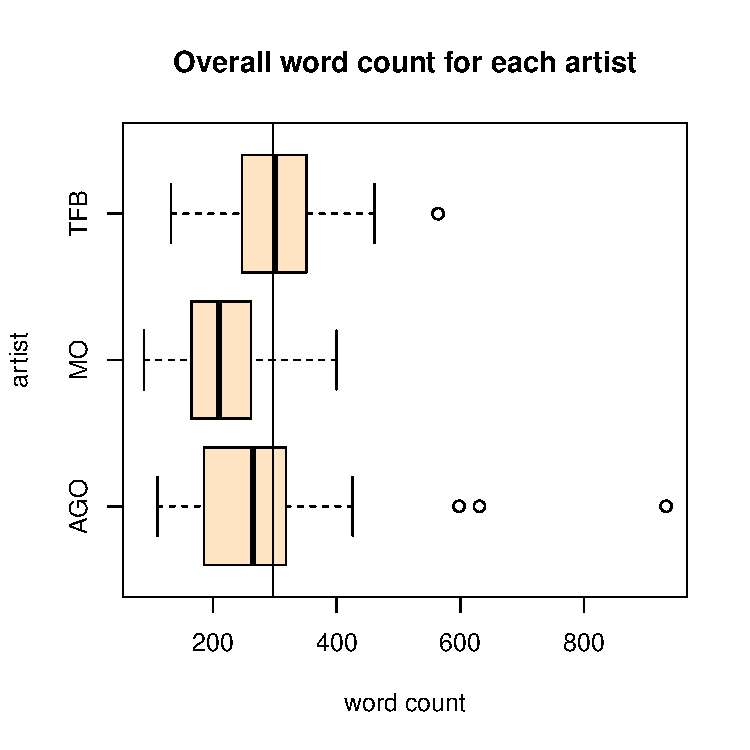
\includegraphics[width=\maxwidth]{figure/unnamed-chunk-4-1} 
\end{knitrout}
\caption{Vertical line represents ``Allentown''} \label{plot2}
\end{figure}

\begin{figure}[H]
\begin{knitrout}\scriptsize
\definecolor{shadecolor}{rgb}{0.969, 0.969, 0.969}\color{fgcolor}
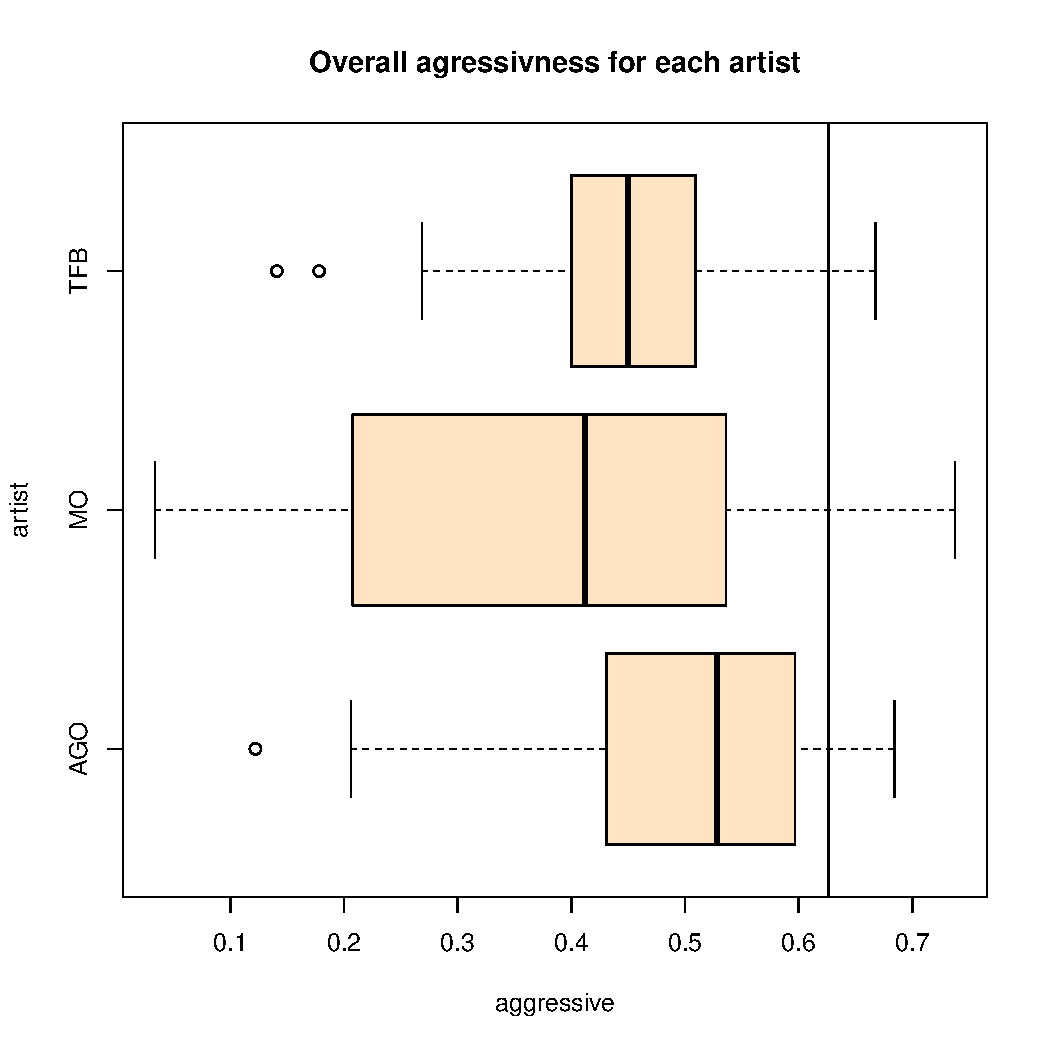
\includegraphics[width=\maxwidth]{figure/unnamed-chunk-5-1} 
\end{knitrout}
\caption{Vertical line represents ``Allentown''} \label{plot3}
\end{figure}

Manchester Orchestra's audio features are the most similar to ``Allentown'' (see Table \ref{allentown.tab}). All Get Out has the second most similar audio features to ``Allentown'' because it has fewer out of range and more in range features than The Front Bottoms has (see Figure \ref{plot.allen}). Manchester Orchestra has the fewest out of range and the most within range features, indicating that this band contributed the most to creating ``Allentown''.

%%%%%%%%%%%%%%%%%%%%%%%%%%%%%%%%%%%%%%%%%%%%%%%%%%%%%%%%%%%%%%%%%%%%%%%%%%%%%%%%
% Bibliography
%%%%%%%%%%%%%%%%%%%%%%%%%%%%%%%%%%%%%%%%%%%%%%%%%%%%%%%%%%%%%%%%%%%%%%%%%%%%%%%%
\vspace{2em}
\begin{tiny}
\bibliography{bib.bib}
\end{tiny}
\end{multicols}

%%%%%%%%%%%%%%%%%%%%%%%%%%%%%%%%%%%%%%%%%%%%%%%%%%%%%%%%%%%%%%%%%%%%%%%%%%%%%%%%
% Appendix
%%%%%%%%%%%%%%%%%%%%%%%%%%%%%%%%%%%%%%%%%%%%%%%%%%%%%%%%%%%%%%%%%%%%%%%%%%%%%%%%
\newpage
\onecolumn
\section{Appendix}
%creating an xtable
% latex table generated in R 4.4.2 by xtable 1.8-4 package
% Tue Feb 25 11:36:04 2025
\begin{table}[ht]
\centering
\begin{tabular}{|l|c|c|c|}
  \hline
Category & All.Get.Out & Manchester.Orchestra & The.Front.Bottoms \\ 
  \hline
Out of Range &  22 &   3 &  30 \\ 
  Outlying &  17 &  11 &  11 \\ 
  Within Range & 158 & 183 & 156 \\ 
   \hline
\end{tabular}
\caption{Comparison of ``Allentown'''s audio features with the range of bands' features} 
\label{allentown.tab}
\end{table}


%creating column plots
\begin{figure}[H] \begin{center}
\begin{knitrout}
\definecolor{shadecolor}{rgb}{0.969, 0.969, 0.969}\color{fgcolor}
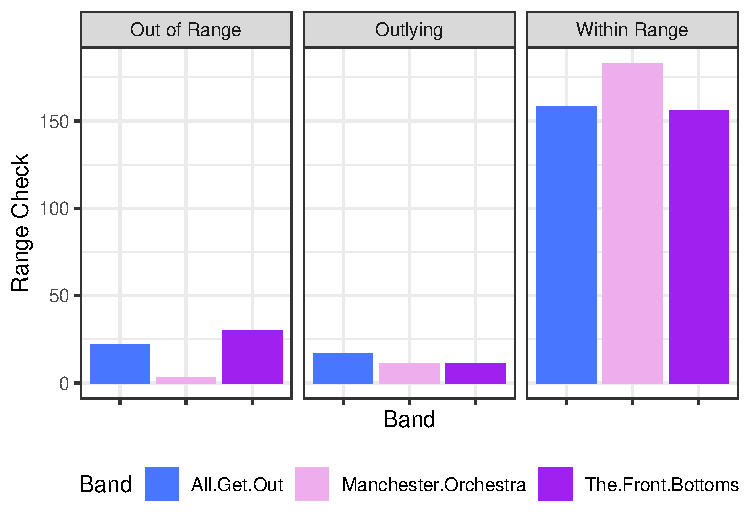
\includegraphics[width=\maxwidth]{figure/unnamed-chunk-6-1} 
\end{knitrout}
\caption{Comparison of ``Allentown'''s audio features with the range of bands' features} \label{plot.allen}
\end{center}
\end{figure}


\end{document}
